\clearpage
\section{Method}
\label{sec:method}

Our method is split into to two parts, the routing algorithm and the accessibility analysis tool.

\subsection{Metric}
\label{subsec:metric}

To evaluate the accessibility in cities, we employ a metric that is an implementation of the 15-minute city concept. The concept measures how fast the access to a variety of important amenities is.
To measure this, we categorize amenities into seven essential services: grocery, education, health, banks, parks, sustenance, and shops.
Each category is populated with Points of Interest (POIs) sourced from OSM, providing a comprehensive database of locations.
Our categorization is based on the work of \cite{olivariAreItalianCities2023} with slight modification and can be seen in Table \ref{tab:categories}.

\begin{table}[ht]
\centering
\caption{Categories and their corresponding OSM tags}
\label{tab:categories}
\footnotesize
\begin{tabular}{|l|l|p{10cm}|}
\hline
\textbf{Category} & \textbf{OSM Key} & \textbf{OSM Value} \\ \hline
Grocery           & shop             & alcohol, bakery, beverages, brewing supplies, butcher, cheese, chocolate, coffee, confectionery, convenience, deli, dairy, farm, frozen food, greengrocer, health food, ice-cream, pasta, pastry, seafood, spices, tea, water, supermarket, department store, general, kiosk, mall \\ \hline
Education         & amenity          & college, driving school, kindergarten, language school, music school, school, university \\ \hline
Health            & amenity          & clinic, dentist, doctors, hospital, nursing home, pharmacy, social facility \\ \hline
Banks             & amenity          & atm, bank, bureau de change, post office \\ \hline
Parks             & leisure          & park, dog park \\ \hline
Sustenance        & amenity          & restaurant, pub, bar, cafe, fast-food, food court, ice-cream, biergarten \\ \hline
Shops             & shop             & department store, general, kiosk, mall, wholesale, baby goods, bag, boutique, clothes, fabric, fashion accessories, jewelry, leather, watches, wool, charity, secondhand, variety store, beauty, chemist, cosmetics, erotic, hairdresser, hairdresser supply, hearing aids, herbalist, massage, medical supply, nutrition supplements, optician, perfumery, tattoo, agrarian, appliance, bathroom furnishing, do-it-yourself, electrical, energy, fireplace, florist, garden centre, garden furniture, fuel, glaziery, groundskeeping, hardware, houseware, locksmith, paint, security, trade, antiques, bed, candles, carpet, curtain, flooring, furniture, household linen, interior decoration, kitchen, lighting, tiles, window blind, computer, electronics, hifi, mobile phone, radio-technics, vacuum cleaner, bicycle, boat, car, car repair, car parts, caravan, fishing, golf, hunting, jet ski, military surplus, motorcycle, outdoor, scuba diving, ski, snowmobile, swimming pool, trailer, tyres, art, collector, craft, frame, games, model, music, musical instrument, photo, camera, trophy, video, videogames, anime, books, gift, lottery, newsagent, stationery, ticket, bookmaker, cannabis, copy shop, dry cleaning, e-cigarette, funeral directors, laundry, moneylender, party, pawnbroker, pet, pet grooming, pest control, pyrotechnics, religion, storage rental, tobacco, toys, travel agency, vacant, weapons, outpost \\ \hline
\end{tabular}
\normalsize
\end{table}

Each service category encapsulates several POIs. 
For instance, the "Parks" category may include multiple locations tagged in OSM as "leisure: park" or "leisure: dog park".

The core of our metric is the determination of temporal proximity to these amenities. 
For each category, we calculate the minimum travel time required to reach at least one POI of that category. 
The metric is then defined as the maximum value among these minimal times across all categories. 
This approach yields a singular measure that reflects the most significant time distance barrier within an urban area, which effectively captures the least accessible category for any given area.
We think that it is beneficial to focus on the least accessible category, as measuring accessibility in cities by averaging accessibility across all categories can mask disparities categories. 
This ensures that the metric is targeted to areas of greatest need. 

This metric is critical in assessing the performance of a neighborhood or a city at large against the 15-minute city ideal. It is not an average of accessibility across services but rather highlights the area of greatest need, providing a clear target for urban development and improvement.

By leveraging this metric, we aim to help city planners to create urban environments that prioritize sustainability, enhance the well-being of residents, and reduce dependency on vehicular transport, thus contributing to the broader goals of efficient urban planning and improved quality of urban life.

% ---- START section about alternative modes
% explain different modes - maybe(?) this belongs to related work
Traditionally, the 15-minute city concept is applied to walking and or cycling and ignores other modes of transport.
Some researchers, in the context of location-based metrics, even go as far to only calculate the bee-line distance to the nearest amenity and ignore the street network altogether \cite{gastnerOptimalDesignSpatial2006}, while most only consider walking \cite{olivariAreItalianCities2023, nicolettiDisadvantagedCommunitiesHave2023}.

We, however, believe that to accurately determine the accessibility of a city, all modes of transport must be considered, and the routing needs to be as realistic as possible.
We will therefore calculate our metric for various combinations of modes of transport, namely driving with a personal car+walking, free-floating bicycle sharing+walking, public transport+walking, free-floating bicycle sharing+public transport+walking, and walking.
The car mode will serve as a baseline metric and show how competitive more sustainable modes of transport are.

Adding potentially fare-based modes of transport poses a challenge, as we need to consider the cost of the trip.
Ignoring the cost of the trip could potentially lead to a misrepresentation of accesibility, as a trip with a high cost might be inaccessible to some people.
To account for this, we will calculate Pareto sets that balance the minimum travel time and the cost of the trip.
% ---- END section about alternative modes



\subsection{Routing Algorithm}
\label{subs:routing_algorithm}

Our routing algorithm is an applied version of MCR with minor variation to make it more suitable in terms of free-floating vehicle sharing.

\subsubsection{Requirements}
\label{subsubsec:requirements}

% requirements on routing algorithm
% - unrestricted
% - multi-modal (must incorporate scheduled networks (public transfer) and an arbitrary number of other unscheduled networks)
% - multi-objective (must be able to incorporate an arbitrary amount of objectives), whose values update based on the previous values and the current edge (either unscheduled network edge or trip between two stops)
% - inter-modal (the different transport modes may be sequenced in any order (not just bicycles for start and end)

In order to fully grasp the potential of the combination of the sustainable modes of transport, we require our routing algorithm to be \textbf{multi-modal}, \textbf{multi-objective}, and \textbf{unrestricted inter-modal}, and run in a reasonable time.

\textbf{Multi-modal} means that our routing algorithms allows multiple modes of transport, including scheduled transport systems, like public transfer and an arbitrary number of unscheduled transport systems, like walking, cycling and driving.
In addition, we require that free-floating vehicle sharing systems are incorporated realistically.
That means, that our routing algorithm must consider that switching to a free-floating vehicle is possible at any location, where a free-floating vehicle is available and parking a free-floating vehicle is possible anywhere where it's allowed.
% note: this extra excludes MCR

\textbf{Multi-objective} means that our algorithm must find all pareto optimal journeys according to an arbitrary amount of objectives.
The algorithm must provide the possibility to update the values of any objective whenever a \textit{movement} occurs.
We define a movement either as an edge traversal in an unscheduled network or a step in the route traversal during McRAPTOR.
In the case of an edge traversal the new objective must be a function of the old objective and the edge weights, formally: \(l' = f(l, w(e))\), where \(l\) and \(l'\) are the old and new labels, respectively, and \(w(e)\) are the weights of the edge that is traversed.
In the case of an update during a step of the route traversal, the new objective must be a function of the old objective (to be continued).

\textbf{Inter-modal} means that the different transport modes may be sequenced in any order.
For example, when considering walking, cycling through a bicycle sharing system and public transport, the algorithm needs to consider journeys with bicycle rides between two consecutive public transport trips.
\textbf{Unrestricted} means that the algorithm fully searches the unscheduled network graphs, and does not pose restrictions like a maximum of 10 minutes walking distance.


% handled:
% dijkstra, mlc, raptor, ultra, mcraptor, mcr
% relate to other algorithms
Both Dijkstra and MLC are not considered due to their impractical runtime.
Furthermore, the need for multi-objective solutions excludes Dijkstra, RAPTOR, and ULTRA.
The requirement for unrestricted inter-modal travel makes RAPTOR and McRAPTOR unsuitable in practical scenarios.
To explain this, let's examine a straightforward example.

Consider the OSM graph of the key regions in Cologne, which comprises 125,176 nodes and 142,074 edges.
For RAPTOR to compute a transitively closed graph, it requires calculating the walking distance between each node.
This computation would yield \(125,176^2 = 15,669,030,976\) edges, a number vastly greater than the original 142,074 edges.

While MCR does support multi-objective solutions with unrestricted inter-modal transfers, it doesn't fully encapsulate the multi-modal concept we require.
Although it theoretically permits various modes of unscheduled transport, it is primarily tailored for station-based vehicle sharing systems.
Our focus, however, is on the increasingly prevalent free-floating systems.
In MCR, unscheduled networks are contracted, leading to the removal of certain nodes.
If an optimal route requires a mode change at a deleted node, MCR will be unable to identify that path.
As a result, MCR is not a viable option for our needs.


In the following section, we detail the modifications made to MCR to tailor it to our requirements.

\subsubsection{Algorithm}
\label{subsubsec:algorithm}

% I/O
The input of our algorithm is a start time and a start node.
The start node may be any node in the OSM network.
The output of our algorithm are the bags for each node in the OSM network.

% Algorithm
% first phase
Our algorithm is split into two phases, which are repeated iteratively.
The algorithm is depicted in Figure \ref{fig:routing_algorithm}.
In the first phase the walking network is explored through the MLC algorithm.
Walking is not considered a trip and there is no upper limit on the walking distance.
In the initial iteration MLC starts with a single label containing the starting values in the bag of the start node.
All other bags are empty.
We run MLC until it converges and retrieve the final bags for each node.

% second phase
In the second phase we explore the public transport network, as well as, all modes of unscheduled travel, except walking.
We do so, because a public transport trip, as well as, a trip with any mode of unscheduled travel, except walking will be counted as a trip.

% second phase - RAPTOR
To explore the public transport network, we run one iteration of McRAPTOR.
To retrieve the proper input bags for McRAPTOR we associate each stop in the public transport network with a node in the unscheduled walking network beforehand.
Then we can use the bags of the nodes in the walking network that are associated with a stop in the public transport network as input for McRAPTOR.

% Second phase - MLC
At the same time, we run MLC again, for each unscheduled mode of transport except walking.
For modes based on free-floating vehicle sharing, we use the bags of nodes in the walking network as an input, where a free-floating vehicle is present.
The output is defined depending on where it is possible to drop off vehicles.
If there are no restrictions the bags of all nodes are used.

% merge
The outputs of the McRAPTOR iteration and all MLC runs are merged.
To do so first the output bags have to be translated into the common nodes of the walking network again.
After that the bags are merged according to the merging rules explained in Section \ref{subsubsec:mcraptor}.

The bags that result the merge are the output of the first iteration and contain all optimal labels after exactly one trip.
To obtain the optimal labels after X trips, both phases have to be repeated X times and the result bags of the second phase in iteration \(i\) are used as the input bags of the first phase in iteration \(i-1\).


\begin{figure}
    \centering
    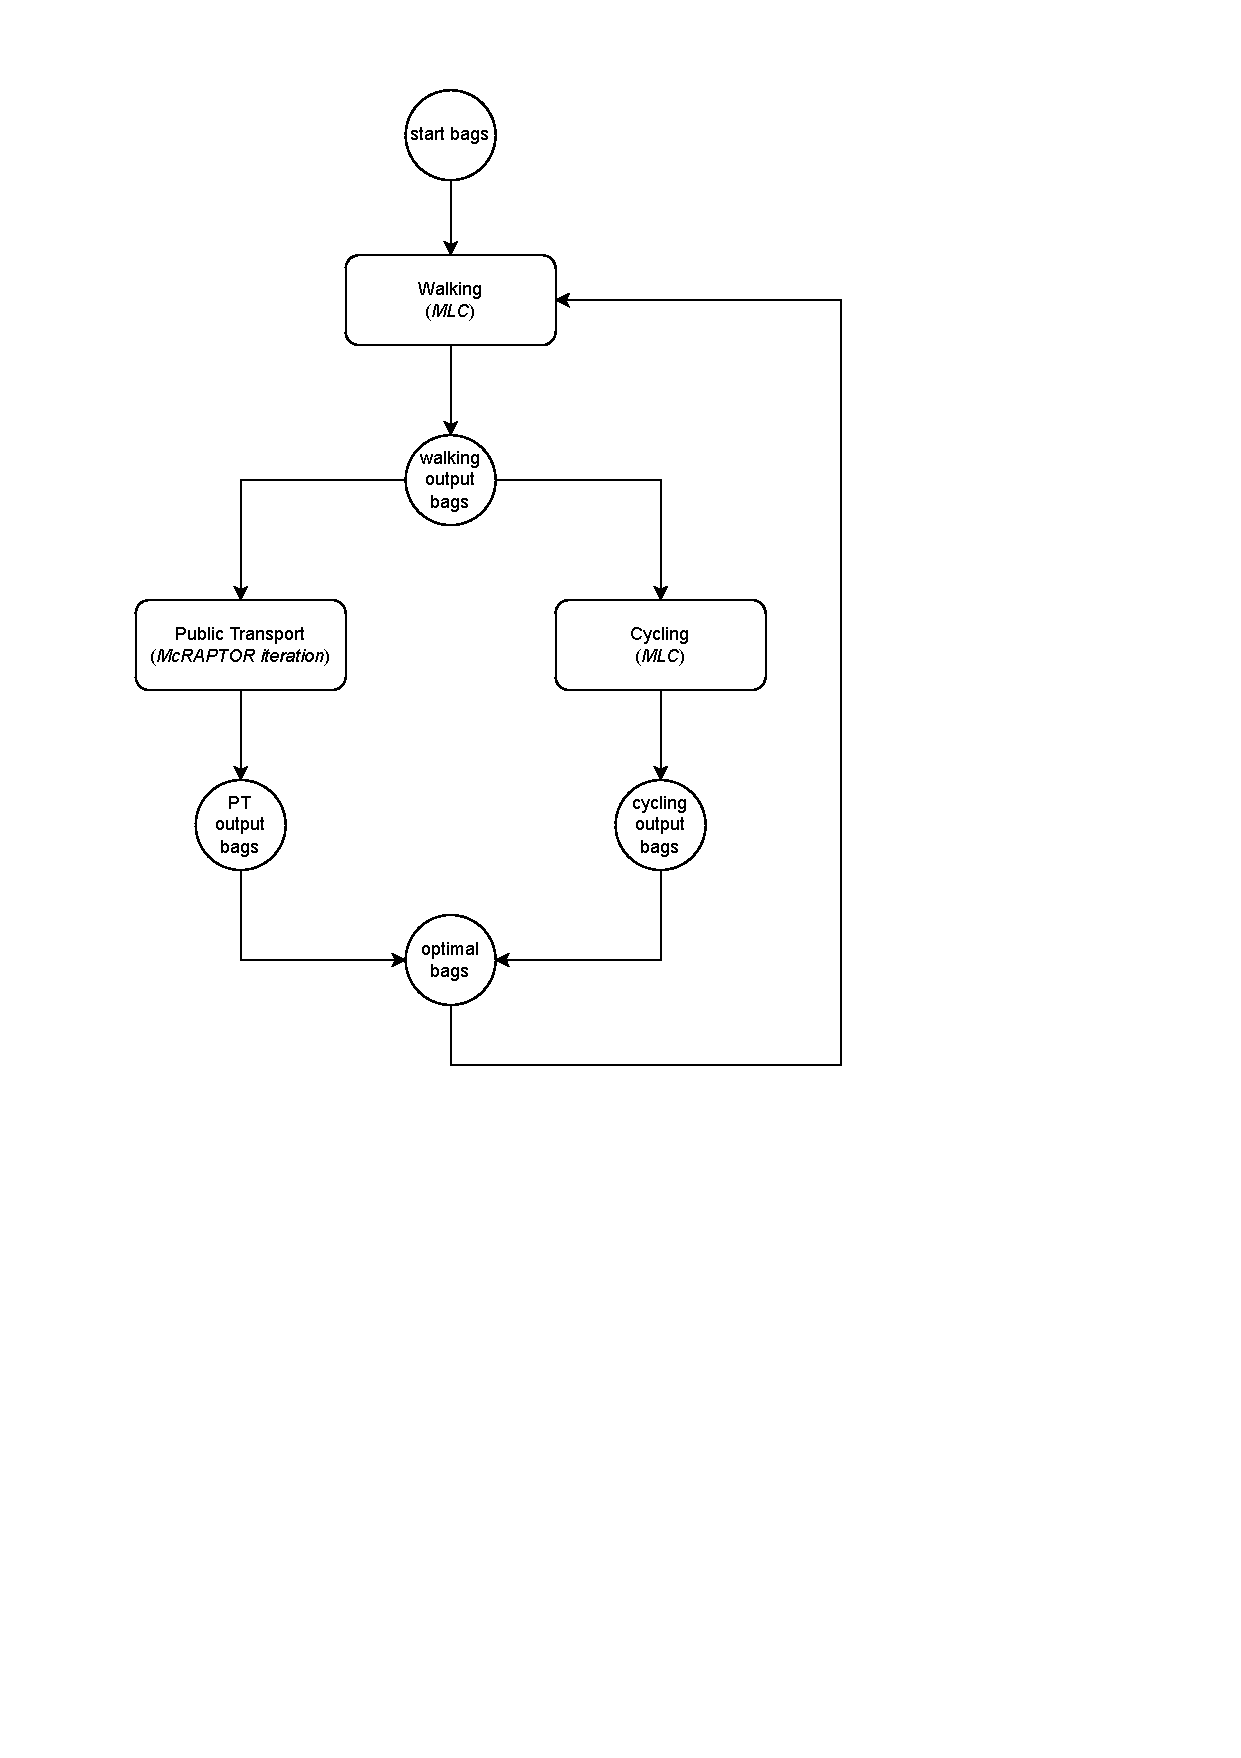
\includegraphics[scale=0.75]{Figures/method/routing_algorithm}
    \caption{Routing Algorithm}
    \label{fig:routing_algorithm}
\end{figure}


\subsection{Accessibility Analysis Tool}
\label{subsec:combining}

We embed the routing algorithm described in Section \ref{subsec:routing_algorithms} in our accessibility analysis routine to compute the metric described in Section \ref{subsec:metric}.

Our accessibility analysis routine consists of three parts: the input routine, the main routine and the metrics routine.

% Input routine
In the input routine we first create an even grid that covers the whole area of interest, for example a city.
To create such a grid, we use H3 \shortcite{H3H3}, which uses hexagons to evenly discretize an area.
Our goal will be to calculate our metric for each hexagon, so that we get detailed spatial information about the accessibility in the area of interest.
The chosen H3 resolution determines the size of these hexagons: a higher resolution means smaller hexagons, enhancing the granularity of our analysis. 
As such, selecting an appropriate H3 resolution is pivotal as it allows us to calculate our metrics for each hexagon with increased spatial accuracy, yielding a detailed spatial dataset that reflects the accessibility variations within the area of interest.
We recommend a resolution of nine, which corresponds to a hexagon edge length of roughly 200 meters, as it is a good compromise between accuracy and computation time.

% START this does not belong here
The underlying street network needs to be larger than the area of interest.
Otherwise, border regions will have a lower accessibility than they should, as the street network is incomplete.
% END this does not belong here

The input routine also filters out uninteresting hexagons.
For, example we filter out hexagons that don't contain any residential areas, as there are no people living there is no need to access any amenities.

Next the input routine gets the centroid of each hexagon and then calculates the euclidean distance between the center and the OSM nodes to find the OSM nodes that is closest to each hexagon's centroid.

The result of the input routine is a set of OSM nodes, for which we want to compute the accessibility.


% Main routine
The main routine calls our routing algorithm described in Section \ref{subsec:routing_algorithms} on each OSM node provided by the input routine.
This results in a set of Bags for each node.

% Metrics routine
The metrics routine processes the bags into Pareto sets, where one entry in the Pareto set is a tuple of the X-minute city metric and the related cost.
%TODO explain metrics routine

